\section{Interpreter}

Der Interpreter führt in der WHILE-""Sprache formulierte Programme aus und stellt eine Schnittstelle zum Debuggen von Programmen zur Laufzeit bereit. Des Weiteren überprüft er mit Hilfe des Evaluators zur Laufzeit die mittels Annotationen in den Programmtext eingebetteten Annotationen. Der Interpreter-""Prozess kann in einem eigenen Thread gestartet werden und teilt anderen Komponenten mit Hilfe des Entwurfsmusters ``Observer'' bei der Ausführung auftretende Ereignisse mit.

\subsection{Die Fassadenklasse \type{Interpreter}}
Die Klasse \type{Interpreter} ist eine Fassade, die innerhalb der Komponente getroffene Entwurfsentscheidungen abstrahiert und die internen Datenstrukturen in ihrer Komplexität reduziert darstellt.

\begin{description}
    \item[Instanziierung] Die Klasse \type{Interpreter} wird mit einer Programmspezifikation initialisiert.

    \item[Ausführung] Mit der Methode \texttt{execute()} wird die Ausführung des im Konstruktur übergebenen Programms gestartet. Der Aufruf kehrt erst nach der Ausführung des kompletten Programms zurück, weshalb es sich anbietet, diese Methode in einem separaten Thread auszuführen. Die öffentlich zugänglichen Datenstrukturen der Klasse Interpreter sind Thread-""Safe und können deshalb auch während der Ausführung modifiziert werden.

    \item[DebugEventListener]
    Mit den Methoden \texttt{add"-DebugEvent"-Listener()} und \texttt{remove"-Debug"-Event"-Listener()} können dem \type{Interpreter}-""Objekt Listener-""Objekte hinzugefügt werden. Diese werden, ähnlich wie im Entwurfsmuster ``Observer'', über Ereignisse bei der Ausführung des Programms benachrichtigt und können unterschiedlich darauf reagieren. Die Klasse \type{Abstract"-Debug"-Event"-Listener} implementiert ``no-op''-""Stubs für alle auftretenden Ereignisse, sodass konkrete Unterklassen nur die von ihnen benötigten Event-""Handler überschreiben müssen.

    Die Event-""Handler werden dabei synchron aufgerufen und können durch Warten die komplette Ausführung blockieren. Auf diese Weise kann ein Debugger Funktionalitäten wie Single-""Step-""Execution oder das Anhalten nach einer fehlgeschlagenen Zusicherungsinstruktion einfach implementieren. Die Interpreter-""Komponente bleibt dadurch weitgehend frei von konkreter Debugger-""Logik.

    \item[Breakpoints]
    Dem Interpreter können Breakpoints in Form von Objekten des Typs \type{Line"-Breakpoint} (bzw.\ \type{Conditional"-Line"-Breakpoint}) hinzugefügt werden. Wird bei der Ausführung die von dem Breakpoint spezifizierte Zeile im Quelltext überschritten, so ruft der Interpreter auf allen ihm hinzugefügten \type{Debug"-Event"-Listener}-""Objekten die Methode \texttt{breakpoint"-Reached()} auf, damit diese das Ereignis behandeln und z.~B.\ die Ausführung unterbrechen können.

    \item[Symbolzuordnung]
    Die Methode \texttt{get"-All"-Symbols()} Gibt die im aktuellen Ausführungskontext gültige Symbolzuordnungstabelle zurück. Symbole werden durch einen String identifiziert und ihr Wert durch die Klasse \type{Value} gekapselt.

    \item[Auswertung von \type{Expression}s]
    Die Methode \texttt{evaluate"-Expression()} wertet die übergebene \type{Expression} im Kontext des aktuellen Programmzustandes aus und gibt den erhaltenen Wert zurück. Um den Programmablauf sowie andere Debug-""Komponenten von diesem externen Eingriff unbeeinträchtigt zu lassen, werden bei der Ausführung der \type{Expression} keine Listener benachrichtigt. Eventuelle Laufzeitfehler bei der Auswertung der \type{Expression} führen zum Werfen einer Exception, die vom Aufrufer gefangen werden kann.
\end{description}

\subsection{Die Visitor-Klasse \type{Interpreter"-AST"-Node"-Visitor}}
Um die im übergebenen AST vorhandenen \type{Statement}s und \type{Expression}s auszuführen bzw.\ auszuwerten, verwendet die Interpreter-""Komponente intern das Entwurfsmuster ``Visitor''. Der Vorteil dieses Entwurfsmusters ist, dass beim ``Besuchen'' der Knoten noch keine Kenntnis über deren Typ nötig ist, denn jeder Knoten ``entscheidet'' selbst, von welcher Methode des Visitors er verarbeitet werden will. \type{Interpreter"-AST"-Node"-Visitor} implementiert deshalb die Schnittstelle \type{AST"-Node"-Visitor}.

Außerdem implementiert die Klasse \type{Interpreter"-AST"-Node"-Visitor} eine Methode \texttt{clone()}. Diese wird intern von der Interpreter-""Fassade verwendet, um bei der Auswertung einer \type{Expression} nicht das ``richtige'' Objekt verwenden zu müssen, sondern alle Operationen mit einer Kopie durchführen zu können. Dies verhindert die Störung des Debug-""Ablaufs durch unerwartete Benachrichtigungen an Listener während der Auswertung.

\subsection{Event-""Handling mit \type{Debug"-Event"-Listener}-""Objekten}
Instanzen von Unterklassen von \type{Abstract"-Debug"-Event"-Listener} behandeln Ereignisse, die bei der Ausführung des Programms auftreten. Die Methoden dieser Klasse werden dabei vom Interpreter synchron aufgerufen, was es dem Listener-""Objekt erlaubt, die Ausführung anzuhalten oder zu verzögern. Dabei müssen nicht alle Methoden überschrieben werden, sodass eine Unterklasse von \type{Abstract"-Debug"-Event"-Listener} auch nur auf eine Teilmenge der definierten Ereignisse reagieren kann. Die abstrakte Klasse \type{Abstract"-Debug"-Event"-Listener} stellt aus diesem Grund für jedes mögliche Ereignis ``no-op''-""Event-""Handler zur Verfügung.

\begin{description}
    \method{public void statementExecuted(Statement statement)}
    Wird vom Interpreter nach jedem Ausführen eines \type{Statement}s aufgerufen.
    \method{public void statementWillExecute(Statement statement)}
    Wird vom Interpreter vor jedem Ausführen eines \type{Statement}s aufgerufen.
    \method{public void executionFailed(Statement statement, InterpreterError error)}
    Wird vom Interpreter nach einer fehlerbedingten Terminierung des Programms aufgerufen~(beispielsweise ausgelöst durch einen Laufzeitfehler).
    \method{public void breakpointReached(Statement statement, LineBreakpoint breakpoint)}
    Wird vom Interpreter aufgerufen, nachdem ein Breakpoint erreicht (und gegebenenfalls die damit assoziierte Bedingung als wahr ausgewertet) wurde.
    \method{public void assertionSucceeded(Assertion assertion)}
    Wird vom Interpreter nach jeder erfolgreichen Ausführung einer Zusicherungsinstruktion aufgerufen.
    \method{public void assertionFailed(Assertion assertion)}
    Wird vom Interpreter nach jeder fehlgeschlagenen Ausführung einer Zusicherungsinstruktion aufgerufen.
    \method{public void expressionEvaluated(Expression expression)}
    Wird vom Interpreter nach jeder Auswertung einer \type{Expression} aufgerufen.
\end{description}

\subsection{Datentyp-""Wrapper-""Klasse \type{Value}}
Die Klasse \type{Value} repräsentiert den Wert einer Variablen im Typsystem des Worthwhile-""Interpreters. Der Typ der Variable kann dabei auch ohne die Verwendung des \texttt{instanceof}-""Operators herausgefunden werden.

\subsection{Fehlerklassen}
\subsubsection{class InterpreterError}
Diese Fehlerklasse dient zur Weitergabe von Fehlern, die im Interpreter bei einer Ausführung des Programms auftreten.

\subsubsection{class StatementInterpreterError extends InterpreterError}
Diese Fehlerklasse enthält neben den in der Klasse \type{Interpreter"-Error} vorhandenen Fehlerinformationen eine Referenz auf das \type{Statement}-""Objekt, an dem der Laufzeitfehler aufgetreten ist.

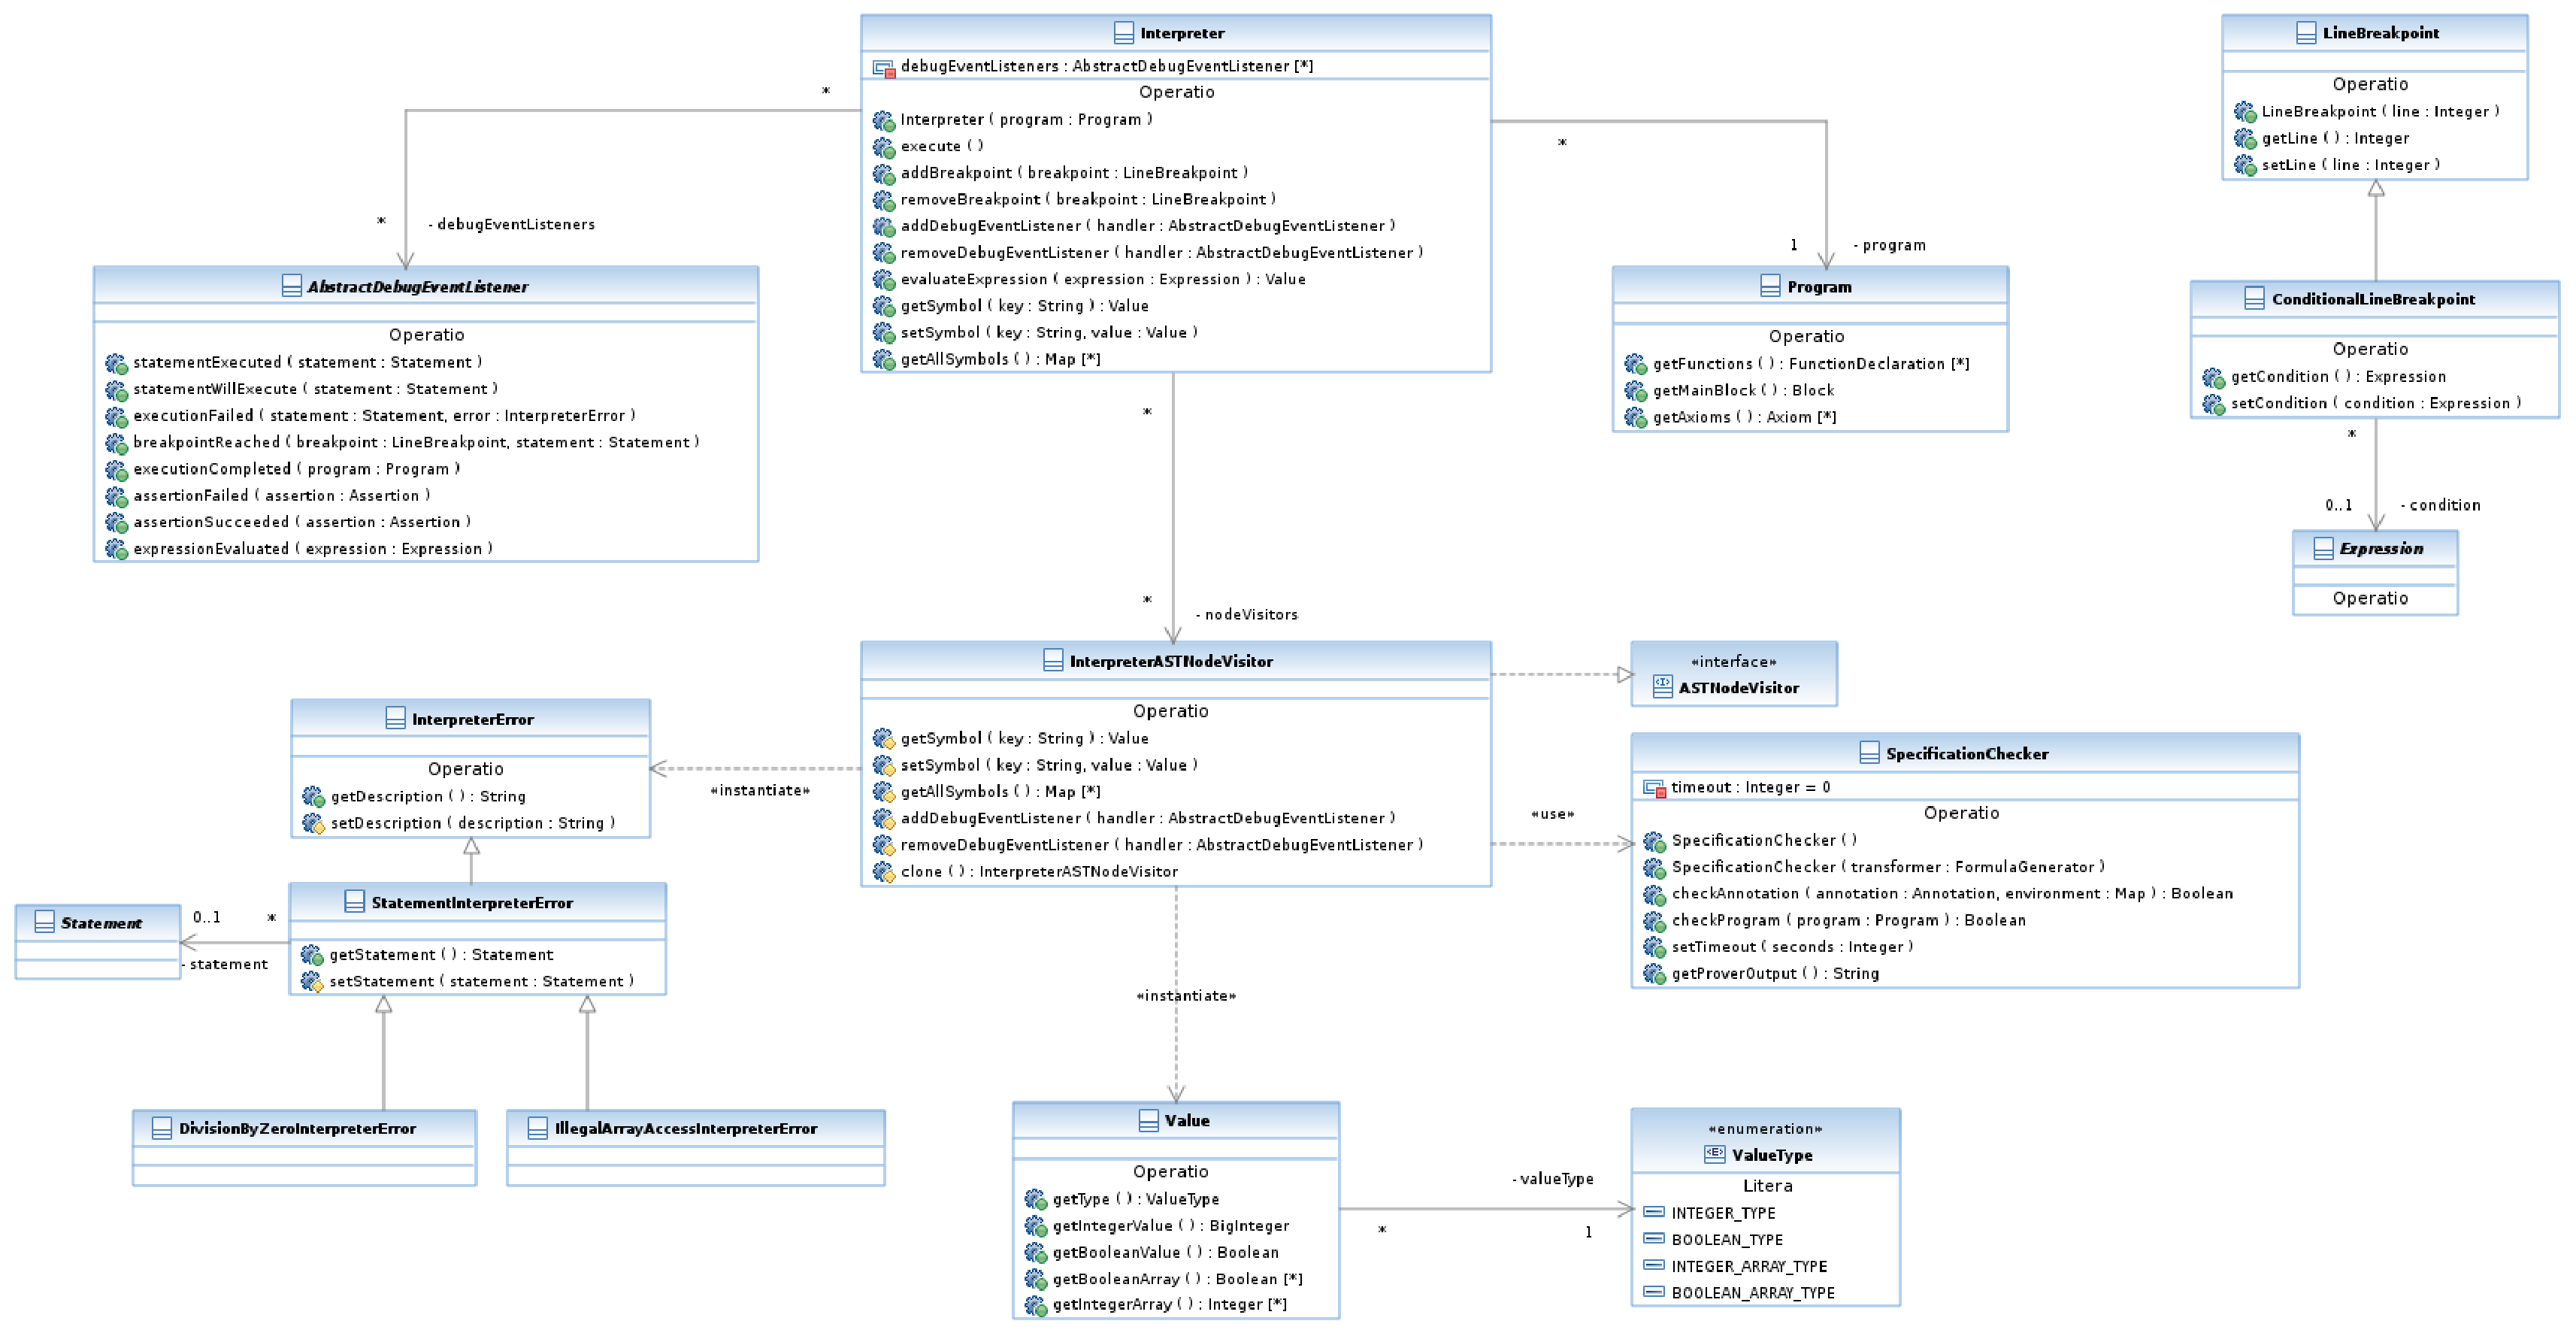
\includegraphics[angle=90,height=\textheight]{diagrams/interpreter_component.pdf}
\newpage

\hspace{-2cm}
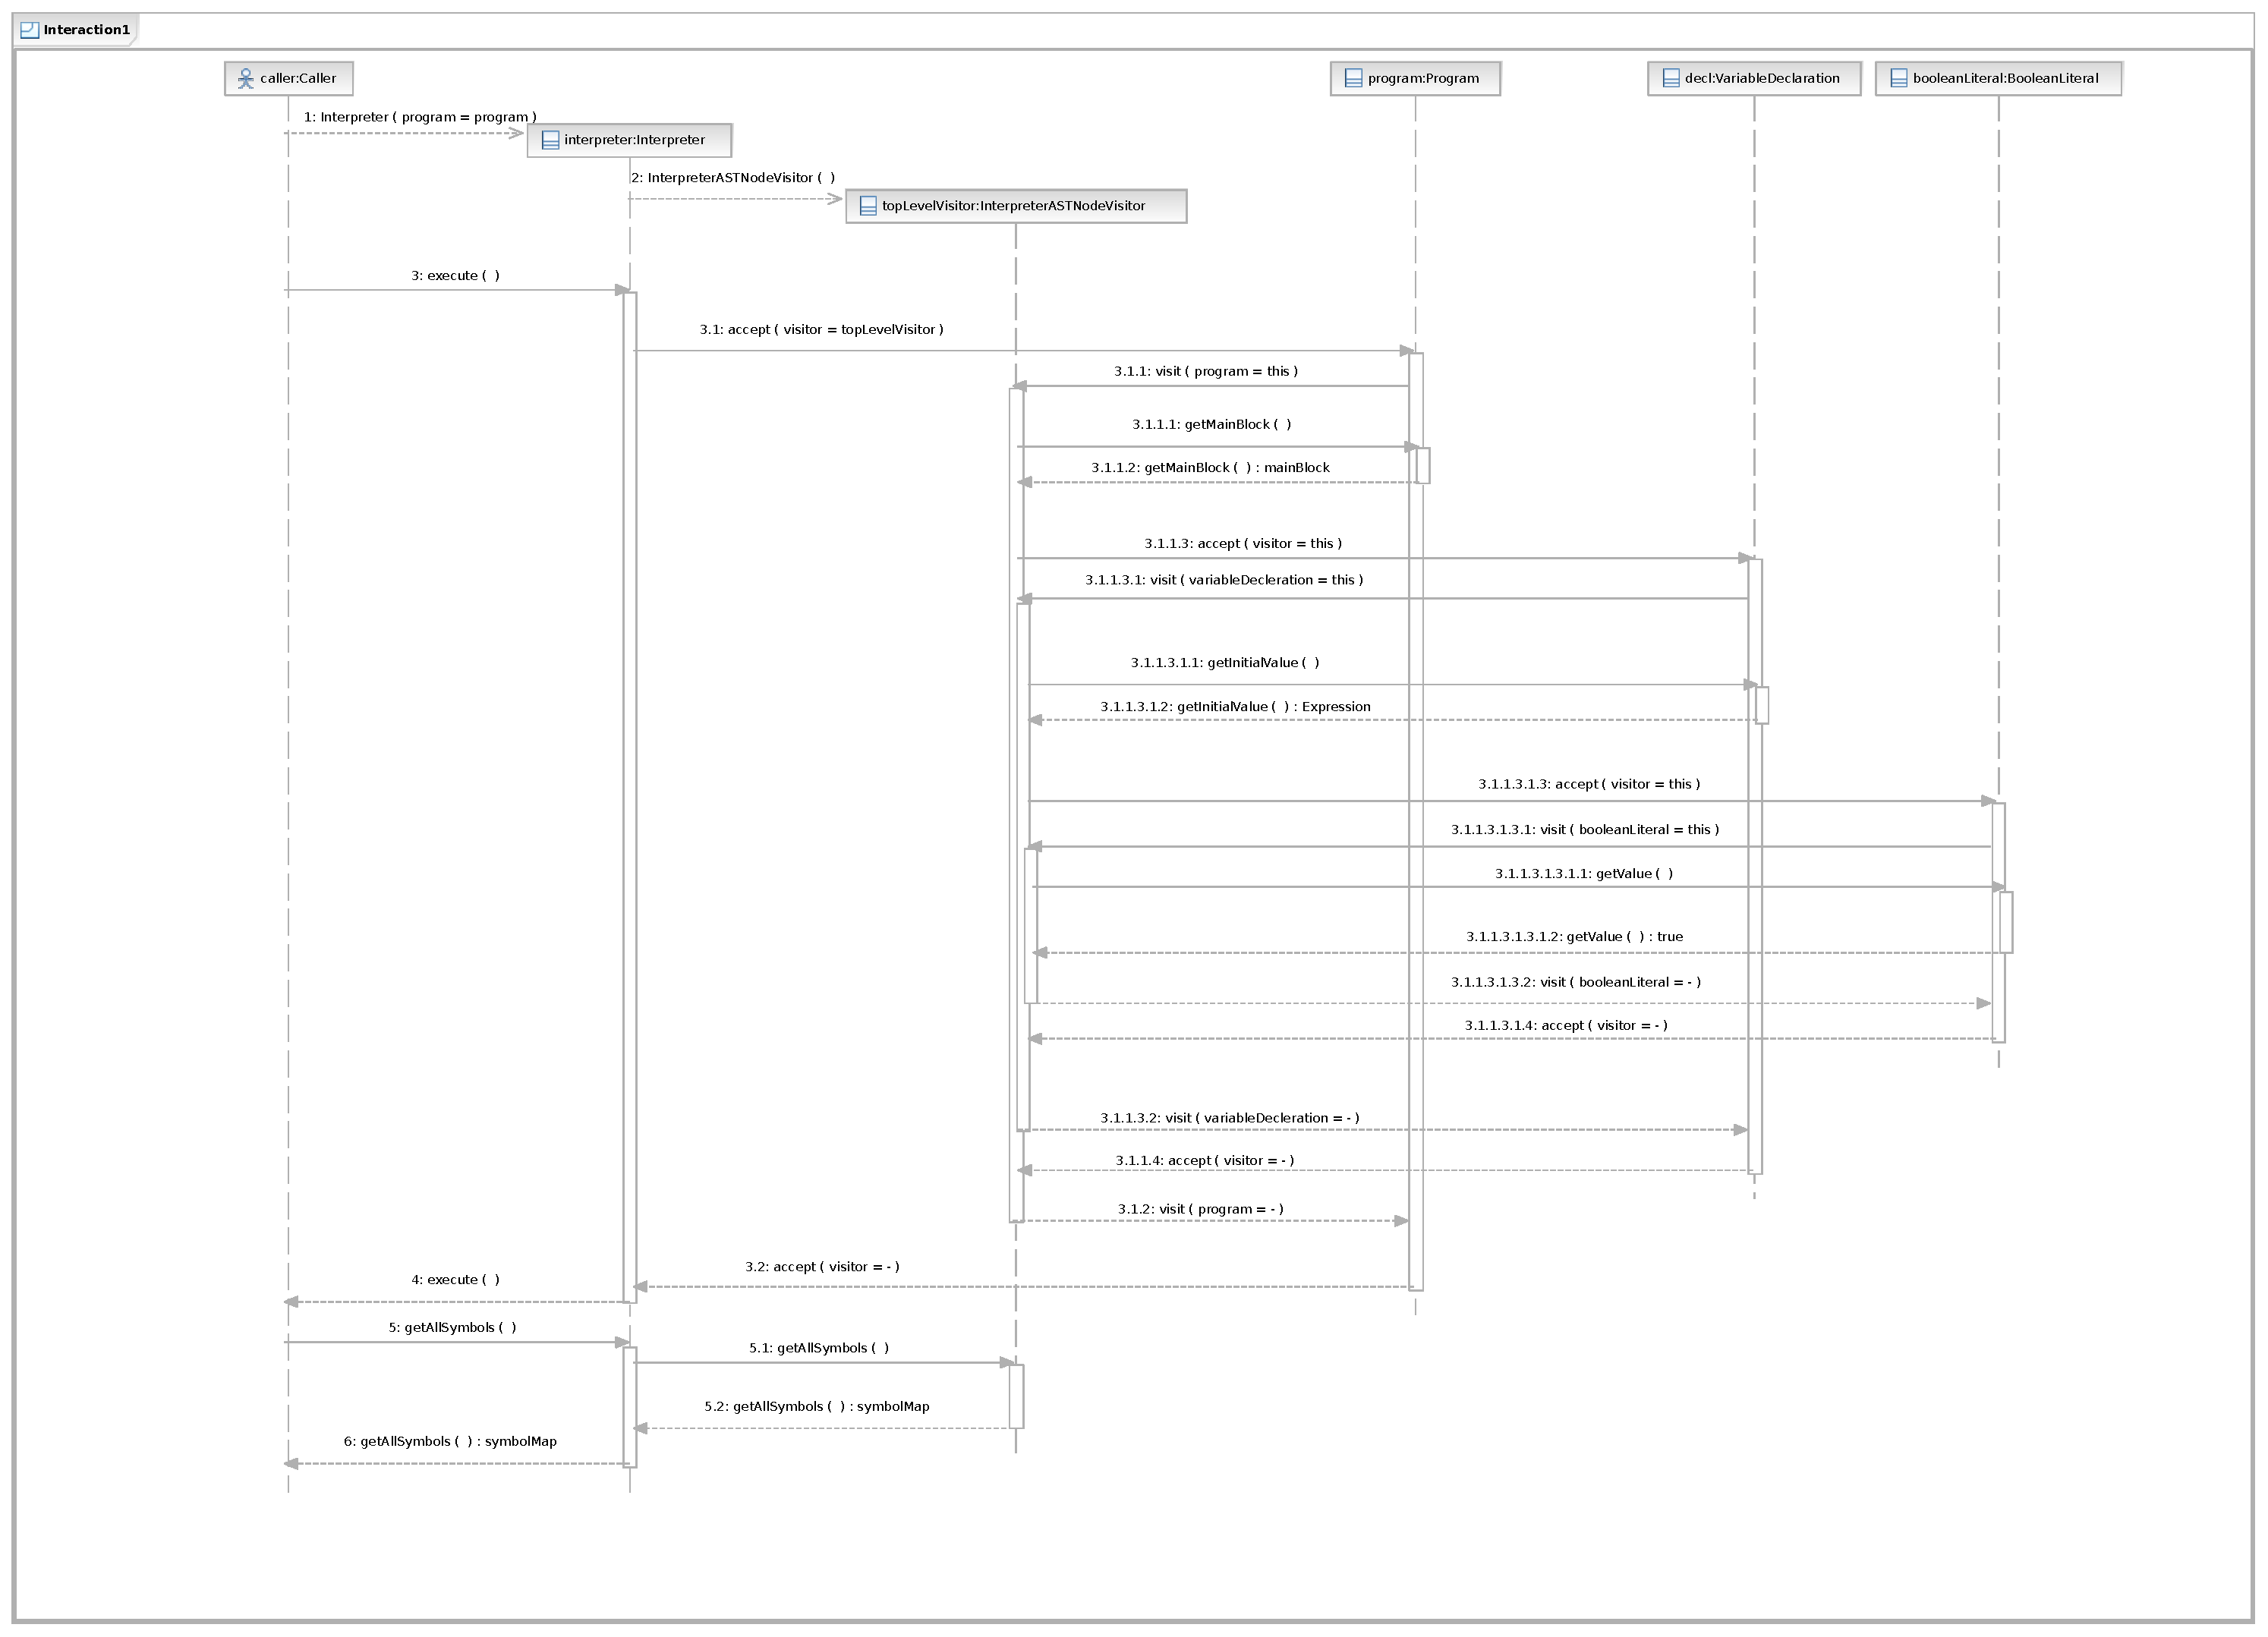
\includegraphics[angle=90,height=\textheight]{diagrams/interpreter_functioncall_sequence.pdf}
